%%%%%%%%%%%%%
% 6 sept 2013 [Jan]: tekeningen herwerkt, fouten verbeterd, OPO
%
% 28/06/2013 [Greetje] Oefeningen toegevoegd
%%%%%%%%%%%%%
\chapter{Inleiding tot de verzamelingenleer}
\label{chap:verzamelingenleer}
\begin{quote}
\textit{`Wat weet jij van deze zaak?' zei de Koning tegen Alice.}

\textit{`Niets,' zei Alice.}

\textit{`\emph{Hoegenaamd} niets?' drong de Koning aan.}

\textit{`Hoegenaamd niets,' zei Alice.}

\textit{`Dit is zeer belangrijk,' zei de Koning, zich tot de jury wendend. Zij stonden juist op het punt dit op hun leien te schrijven, toen het Witte Konijn interrumpeerde.}

\textit{`\emph{On}belangrijk, bedoelt Uwe Majesteit natuurlijk,' zei hij op zeer respectvolle toon, maar hij fronste en grimaste terwijl hij sprak.}

\textit{`Natuurlijk, onbelangrijk bedoelde ik,' zei de Koning haastig, en op gedempte toon vervolgde hij in zichzelf: `belangrijk -- onbelangrijk -- onbelangrijk -- belangrijk --' alsof hij naging welk woord het beste klonk.}

          Uit `Alice in Wonderland' -- Lewis Carroll
\end{quote}

\newpage
\section{Geschiedenis}
`Verzamelingenleer' is de tak van de wiskunde die zich bezighoudt met de studie van `verzamelingen'. Een verzameling is een samenraapsel van objecten die \'e\'en geheel vormen, dingen die een zelfde eigenschap bezitten, dingen die zich op dezelfde manier onderscheiden van de rest. Zo is een klas een verzameling leerlingen die op hetzelfde tijdstip over hetzelfde vak les krijgen.


Fundament in de verzamelingenleer is de idee van `element zijn van', `behoren tot'. De verschillende elementen vormen samen terug \'e\'en geheel, namelijk de verzameling.

De grondslagen van de verzamelingenleer werden gelegd door de Duitse 
wiskundige G. Cantor (1845--1918, figuur~\ref{fig:cantor}). 
Cantor ontwikkelde een formele definitie van `verzameling'. 
Hij definieerde ook bewerkingen met verzamelingen: unie, doorsnede, 
verschil en product. Een belangrijk deel van de moderne wiskunde is 
gebaseerd op Cantors definitie van verzameling.  Een functie is 
bijvoorbeeld een  verzameling van paren getallen.

\begin{figure}[htbp]
\centering
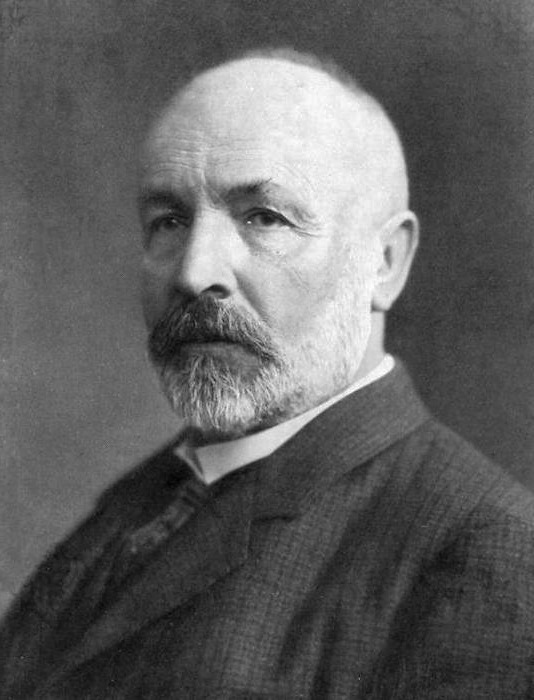
\includegraphics[width=0.5\textwidth]{figuren/verzamelingen_relaties/cantor.jpg}
\caption{Georg Ferdinand Ludwig Philipp Cantor, grondlegger van de moderne verzamelingenleer}
\label{fig:cantor}
\end{figure}
Ook voor computerwetenschappen is verzamelingenleer belangrijk. We geven enkele voorbeelden.  In een programmeertaal is een datatype een verzameling van elementen die op dezelfde manier in het geheugen van het systeem opgeslagen worden en waar je dezelfde bewerkingen op kan toepassen. Als je een lus programmeert, neemt de controle-variabele alle waarden aan binnen een bepaalde verzameling (figuur~\ref{fig:lusScilab}). Bij registratie op een website controleert de webserver of de gekozen gebruikersnaam reeds behoort tot de bestaande verzameling van gebruikersnamen. Bij het inloggen op je favoriete spelletjessite wordt je gebruikersnaam gekoppeld aan de verzameling resultaten die je reeds boekte. Een figuur is een verzameling punten en lijnen. Last but not least, het moderne database design is gebaseerd op de verzamelingenleer: in een tabel zijn de gegevens element van een kolom (figuur~\ref{fig:database}). 

De leerstof die in dit hoofdstuk behandeld wordt, heb je expliciet nodig in de OPO's `Toegepaste wiskunde 3' (2TX), `Technieken van datamodellering' (1TX) en `Databanken' (2TX).

\begin{figure}
\begin{verbatim}
function y=faculteit(n)
    y=1
    for i=1:n
        y=y*i
    end
endfunction
\end{verbatim}
\caption{In Scilab duidt $1:n$ op de  verzameling  $1,2,\dots,n$ waarbij $i$ eerst de waarde van het kleinste element aanneemt.}
\label{fig:lusScilab}
\end{figure}

\begin{figure}[htbp]
\centering
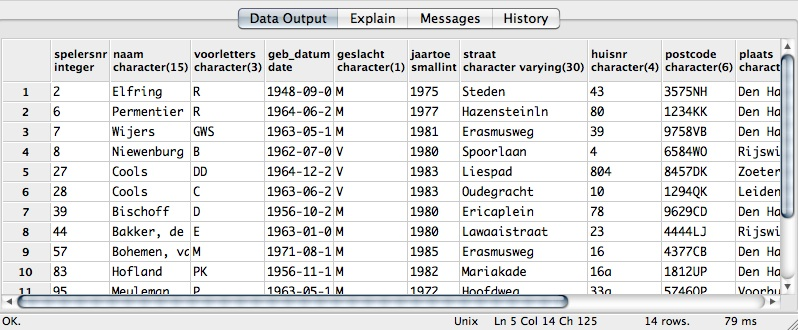
\includegraphics[width=\textwidth]{figuren/verzamelingen_relaties/database.jpg}
\caption{Database als toepassing op verzamelingenleer}
\label{fig:database}
\end{figure}

\section{Verzamelingen en elementen}
\subsection{Definities}
\begin{quote}
Een verzameling\index{verzameling} is een collectie objecten die een geheel vormen.
\end{quote}
We geven enkele voorbeelden van objecten die een verzameling vormen.
\begin{itemize}
  \item de kleuren van de regenboog 
  \item de positieve gehele getallen kleiner dan 10
  \item de zandkorrels van de zee
  \item de OPO's die je dit jaar opneemt in je jaarprogramma 
  \item de gebruikersnamen verbonden aan een beveiligde website
\end{itemize}

De objecten die de verzameling vormen noemen we \emph{elementen}\index{element}. We benoemen elementen met kleine letters en verzamelingen met hoofdletters. Als een element $a$ behoort tot de verzameling $X$ noteren we dat met $a \in X$. Het symbool $\in$\index{\ensuremath{\in}} lezen we als `behoort tot' of `is element van'. Als $a$ \emph{niet} behoort tot $X$ noteren we dat met $a\not \in X $\index{\ensuremath{\not\in}}.

Een verzameling kan een willekeurig aantal elementen hebben: \'e\'en, honderd of vijf miljard. Sommige verzamelingen hebben oneindig veel elementen (bijvoorbeeld de verzameling van de gehele getallen). Het is ook mogelijk dat een verzameling nul (geen) elementen bevat (bijvoorbeeld de verzameling van levende mensen ouder dan 200 jaar). De verzameling met nul elementen noemen we de \emph{lege verzameling}\index{lege verzameling}\index{verzameling!leeg}. We gebruiken voor de lege verzameling het symbool $\emptyset$\index{\ensuremath{\emptyset}}.

Er bestaat \emph{geen rangorde} tussen de elementen van een verzameling: er is geen element `eerst' of `laatst'. De elementen zijn steeds \emph{ongeordend}. 

\subsection{Verzamelingen voorstellen}
Er bestaan verschillende manieren om een verzameling voor te stellen. Je kan een verzameling grafisch voorstellen in een venndiagram, je kan de elementen \'e\'en voor \'e\'en opsommen of je kan de voorwaarden omschrijven waaraan een element moet voldoen om tot de verzameling te behoren.

\subsubsection{Venndiagram}
Venndiagrammen\index{Venndiagram} zijn genoemd naar de Engelse wiskundige J. Venn (figuur~\ref{fig:venn}), die ze omstreeks 1880 bedacht. Het is een grafische manier om een verzameling voor te stellen. De verzameling zelf wordt begrensd door een gesloten kromme (ellips, cirkel, rechthoek, \dots). De elementen worden aangeduid met punten waarbij eventueel hun naam of waarde wordt genoteerd (zie figuur~\ref{fig:venn1}). Als de verzameling te veel elementen bevat om ze allemaal te tekenen, worden er slechts enkele elementen expliciet getekend en worden de andere elementen samengevat in drie puntjes (`$\cdots$') (zie figuur~\ref{fig:venn2}).

\begin{figure}[htbp]
\centering
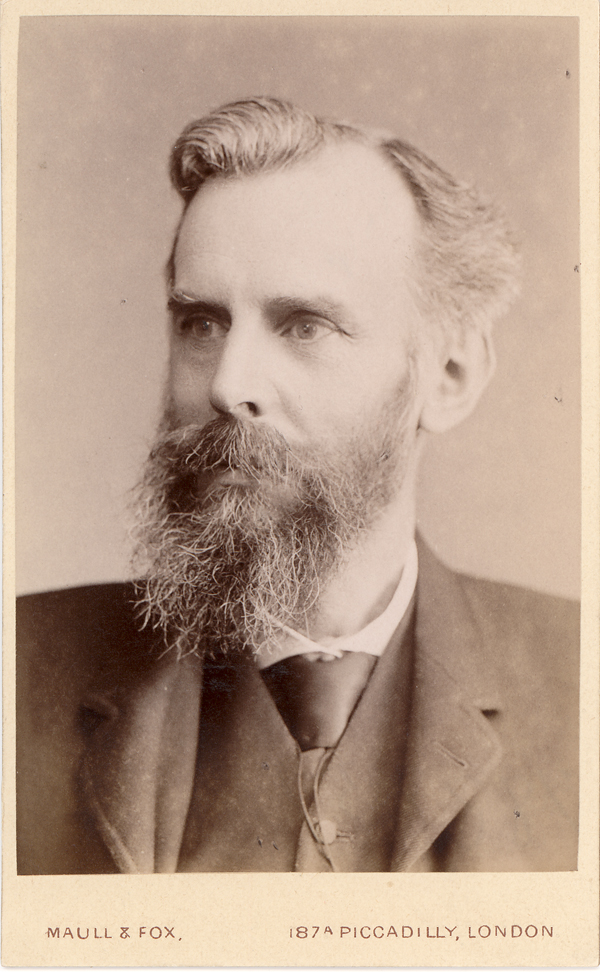
\includegraphics[width=0.5\textwidth]{figuren/verzamelingen_relaties/venn.jpg}
\caption{John Venn (1834--1923)}
\label{fig:venn}
\end{figure}

\begin{figure}[htbp]
\centering
\subfloat[positieve gehele getallen kleiner dan 10]{
    %getallen kleiner dan 10
\begin{tikzpicture}
\draw[outline] (0,0) ellipse [x radius=1.5cm, y radius=2cm] node at (1,2) {$A$};
\draw[fill] (0.7,0.8) \bol node[above] {$1$};
\draw[fill] (-0.6,0.9) \bol node[above] {$2$};
\draw[fill] (0,1) \bol node[above] {$3$};
\draw[fill] (0.3,0.2) \bol node[above] {$4$};
\draw[fill] (-0.9,0.2) \bol node[above] {$5$};
\draw[fill] (-0.9,-0.9) \bol node[above] {$6$};
\draw[fill] (0.4,-.7) \bol node[above] {$7$};
\draw[fill] (1.1,-0.8) \bol node[above] {$8$};
\draw[fill] (0,-1.3) \bol node[above] {$9$};
\end{tikzpicture}

    \label{fig:venn1}
}\qquad
\subfloat[de gehele getallen kleiner dan 0]{
    %%regenboogkleuren
\begin{tikzpicture}
\draw[outline] (0,0) ellipse [x radius=1.5cm, y radius=2cm] node at (1,2) {$A$};
\draw[fill] (0.5,0.8) \bol node[above] {$-1$};
\draw[fill] (-0.6,0.3) \bol node[above] {$-2$};
\draw[fill] (0.7,0) \bol node[above] {\ldots};
\draw[fill] (0.1,-1.1) \bol node[above] {$-3$};
\end{tikzpicture}
    \label{fig:venn2}
}
\caption{Grafische voorstelling van verzameling met een venndiagram}
\label{fig:venndiagram}
\end{figure}

\subsubsection{Opsomming}\index{opsomming}
Als een verzameling niet te veel elementen bevat, kunnen we gewoon alle elementen noteren. Om aan te duiden dat het gaat om een verzameling, omgeven we de elementen met de symbolen $\{$ en $\}$. We geven enkele voorbeelden:
\begin{itemize}
\item $\{0,1,2,3,4,5,6,7,8,9\}$ is de verzameling van positieve gehele getallen kleiner dan 10
\item $\{ \mathrm{ rood, oranje, geel, groen, blauw, indigo, violet}\}$ is de verzameling van kleuren van de regenboog
\end{itemize}
Als het aantal elementen te groot is voor een volledige opsomming, worden soms slechts enkele elementen opgesomd. De overige elementen worden met drie puntjes aangeduid. Het moet dan wel duidelijk zijn uit de beperkte opsomming waarvoor de puntjes staan. Bijvoorbeeld
\begin{itemize}
\item $\{-1,-2,-3,-4,\cdots \}$ is de verzameling van de gehele getallen kleiner dan 0.
\end{itemize}

Het is niet belangrijk in welke volgorde de elementen opgesomd worden. Je mag hetzelfde element ook meerdere keren laten voorkomen in de opsomming. Bijvoorbeeld: de verzameling voorgesteld door $\{1,2,3\}$ bevat dezelfde elementen als de verzameling voorgesteld door $\{3,2,2,1\}$.

\subsubsection{Omschrijving}
De opsomming met puntjes is niet altijd eenduidig. In zo'n gevallen is het beter de verzameling te defini\"eren met een omschrijving. We geven enkele voorbeelden.
\begin{itemize}
\item $\{x\mid x \in \integers ~\mathrm{ en }~ x<0\}$: de verzameling van gehele getallen kleiner dan 0. Deze verzameling wordt soms ook kort genoteerd als $\{x \in \integers \mid x<0\}$
\item $\{ 2\cdot x +1 \mid x \in \nat\}$: de verzameling van oneven gehele getallen groter dan 0
\end{itemize}
We lezen bovenstaande notatie als `de verzameling van $x$-en \emph{waarvoor geldt} dat $x$ element is van $\integers$ en $x$ kleiner is dan 0'.

\subsection{Gelijke verzamelingen}
Twee verzamelingen $X$ en $Y$ zijn \emph{gelijk}\index{verzameling!gelijkheid} als elk element van $X$ ook tot $Y$ behoort en omgekeerd. We noteren $X=Y$. Voorbeelden:
\begin{itemize}
\item $\{1,2,3,4 \}=\{4,3,2,1 \}$
\item $\{\mathrm{rood, geel, groen} \}=\{\mathrm{groen, rood, geel, groen} \}$
\item $\{x\mid x \in \integers ~\mathrm{ en }~ x<0 ~\mathrm{ en }~ x\geqslant -4\}=\{-1,-2,-3,-4 \}$:
\end{itemize}
Als twee verzamelingen niet gelijk zijn, schrijven we $X \not = Y$.

\subsection{Deelverzameling}\index{deelverzameling}\index{verzameling!deel-}
Als alle elementen van $X$ ook element zijn van $Y$, dan noemen we $X$ een \emph{deelverzameling} van $Y$. We noteren $X\subset Y$. Bijvoorbeeld
\begin{itemize}
\item $\{1,2,3 \}\subset \{ 1,2,3,4,5,6,7 \}$
\item $\{x \mid x ~\mathrm{is~student~van~1TX3/1} \} \subset \{x \mid x ~\mathrm{is~student~van~KHLeuven} \}$
\end{itemize}

Omdat de lege verzameling geen element bevat, is de lege verzameling  deelverzameling van alle andere verzamelingen. Elke verzameling is ook deelverzameling van zichzelf. Dus geldt voor elke verzameling $X$ dat $\emptyset \subset X$ en $X \subset X$.

\subsection{Conjuncte en disjuncte verzamelingen}
Twee verzamelingen zijn \emph{conjunct}\index{conjunct} als ze minstens \'e\'en element gemeenschappelijk hebben.
Twee verzamelingen zijn \emph{disjunct}\index{disjunct} als ze geen enkel element gemeenschappelijk hebben. Bijvoorbeeld
\begin{itemize}
  \item $\{ a, b, c \}$ en $\{ b, c, d \}$ zijn conjunct want ze hebben de elementen $b$ en $c$ gemeenschappelijk (figuur~\ref{fig:conjunct}) 
  \item  $\{ a, b, c \}$ en $\{ d, e, f \}$ zijn disjunct (figuur~\ref{fig:disjunct})
\end{itemize}
\begin{figure}
  \centering
  \subfloat[$\{ a, b, c \}$ en $\{ b, c, d \}$ zijn conjunct]{
      %conjuncte verzamelingen
\begin{tikzpicture}
    \draw[outline] \firstcircle node at (-0.5,2.2) {$A$};
    \draw[outline] \tweedecirkel node at (1.7,2.2) {$B$};
    \draw[fill] (-0.9,0) \bol node[above] {$a$};
    \draw[fill] (0.7,0.6) \bol node[above] {$b$};
    \draw[fill] (0.6,-0.9) \bol node[above] {$c$};
    \draw[fill] (2,0.3) \bol node[above] {$d$};
\end{tikzpicture}

      \label{fig:conjunct}
  }\qquad
  \subfloat[$\{ a, b, c \}$ en $\{ d, e, f \}$ zijn disjunct]{
      %disjuncte verzamelingen
\begin{tikzpicture}
    \draw[outline] \firstcircle node at (-0.5,2.2) {$A$};
    \draw[outline] \tweedecirkel node at (1.7,2.2) {$B$};
    \draw[fill] (-0.9,0) \bol node[above] {$a$};
    \draw[fill] (-0.7,0.9) \bol node[above] {$b$};
    \draw[fill] (-0.6,-0.9) \bol node[above] {$c$};
    \draw[fill] (2,0.7) \bol node[above] {$d$};
    \draw[fill] (2.1,-0.1) \bol node[above] {$e$};
    \draw[fill] (1.8,-0.9) \bol node[above] {$f$};
\end{tikzpicture}

      \label{fig:disjunct}
  }
  \caption{Conjuncte en disjuncte verzamelingen}
  \label{fig:conjunct-disjunct}
\end{figure}

\subsection{Verzameling van verzamelingen}
In alle voorgaande voorbeelden zijn de elementen van een verzameling eenvoudige objecten zoals getallen en kleuren. Een element kan echter op zijn beurt \emph{ook} een verzameling zijn. We spreken dan van een verzameling van verzamelingen. Bijvoorbeeld
\begin{itemize}
  \item $\{\{1\},\{2\},\{3\} \}$ is de verzameling met als elementen $\{1\}$, $\{2\}$ en $\{3\}$.
  \item $\{ \emptyset, \{\mathrm{a}\}, \{\mathrm{b}\}, \{\mathrm{a},\mathrm{b}\}\}$ is de verzameling die alle deelverzamelingen van $\{ \mathrm{a},\mathrm{b}\}$ bevat.
\end{itemize}
Let dus goed op dat je verzamelingen correct noteert. 
Immers,\\ $\{1,2,3 \}\not = \{\{ 1\},\{2 \},\{3 \} \}$.



\newpage
\section{Bewerkingen}
Bij getallen kan je  uit twee getallen een derde getal maken door ze  op te tellen en/of te  vermenigvuldigen. Ook bij verzamelingen zijn er een aantal bewerkingen. We bespreken hier unie, doorsnede, verschil en complement. Het product van verzamelingen bespreken we in de volgende sectie.

\subsection{Unie of vereniging}\index{unie}\index{\ensuremath{\union}}
Bij de unie van twee verzamelingen worden de elementen van beide verzamelingen samengevoegd tot \'e\'en nieuwe verzameling. Dubbels worden daarbij weggelaten. We noteren met $X \union Y$ (figuur~\ref{fig:unie_algemeen}). 
\begin{equation*}
X \union Y =\{x \mid x\in X ~\mathbf{of}~x\in Y \}
\end{equation*}

Bijvoorbeeld
\begin{itemize}
\item Als $X=\{\mathrm{a},\mathrm{b},\mathrm{c}\}$ en $Y=\{\mathrm{c},\mathrm{d},\mathrm{e}\}$, dan is $X\union Y=\{\mathrm{a},\mathrm{b},\mathrm{c},\mathrm{d},\mathrm{e}\}$ (figuur~\ref{fig:unie_voorbeeld}).
\item $X=\{a \mid a\in \nat ~\mathrm{en}~a\leqslant 10\}$ en $Y=\{a \mid a\in \nat ~\mathrm{en}~a>10\}$ geeft $X\union Y=\nat$
\end{itemize}
\begin{figure}[htbp]
\centering
\subfloat[Unie van verzamelingen: algemeen]{
%unie algemeen
\begin{tikzpicture}[thick]
\fill[fill=gray!30] \firstellipse;
\fill[fill=gray!30] \secondellipse; 
\draw \firstellipse node at (35:3.7cm) {$Y$};
\draw \secondellipse node at (145:3.7cm) {$X$};
\end{tikzpicture}
    \label{fig:unie_algemeen}
}\qquad
\subfloat[$\{\mathrm{a},\mathrm{b},\mathrm{c}\} \union \{\mathrm{c},\mathrm{d},\mathrm{e}\}$]{
%unievoorbeeld
\begin{tikzpicture}[thick]
\fill[fill=gray!30] \firstellipse;
\fill[fill=gray!30] \secondellipse;
\draw \firstellipse node at (35:3.7cm) {$Y$};
\draw \secondellipse node at (145:3.7cm) {$X$};

\draw[fill] (-2,1.4) \bol node [above] {a};
\draw[fill] (-1.7,0.6) \bol node [above] {b};
\draw[fill] (0,1) \bol node [above] {c};
\draw[fill] (2,1.4) \bol node [above] {d};
\draw[fill] (1.7,0.5) \bol node [above] {e};
\end{tikzpicture} 
    \label{fig:unie_voorbeeld}
}
\caption{Unie van twee verzamelingen}
\end{figure}


\subsection{Doorsnede of intersectie}\index{doorsnede}\index{\ensuremath{\intersection}}
De doorsnede van twee verzamelingen $X$ en $Y$ bevat enkel die elementen die tot $X$ \emph{en} tot $Y$ behoren. We noteren de doorsnede met $X\intersection Y$ (figuur~\ref{fig:doorsnede_algemeen}).
\begin{equation*}
X\intersection Y =\{a \mid a\in X ~\mathbf{en}~a\in Y \}
\end{equation*}

Bijvoorbeeld
\begin{itemize}
\item $X=\{a \mid a\in \nat_0 ~\mathrm{en}~a\leqslant 8\}$ en $Y=\{a \mid a\in \nat ~\mathrm{en}~a>5\}$ geeft $X\intersection Y=\{6,7,8\}$ (figuur~\ref{fig:doorsnede_voorbeeld})
\item Stel dat een wachtwoord pas geldig is als het meer dan 5 karakters telt, waaronder minstens één cijfer. Dan hebben we het volgende: \\
$X=\{a\mid a ~\mathrm{is~een~woord~langer~dan~5~karakters} \}$ en \\$Y=\{a\mid a~ \mathrm{is~een~woord~dat~ook~een~cijfer~bevat } \}$ geeft \\
$X\intersection Y=\{a \mid a~\mathrm{is~een~geldig~wachtwoord} \}$

\end{itemize}

\begin{figure}[htbp]
\centering
\subfloat[Doorsnede van verzamelingen: algemeen]{
%doorsnede algemeen
\begin{tikzpicture}[thick]
\begin{scope}
    \clip \firstellipse;
    \fill[fill=gray!30] \secondellipse;
\end{scope}
\draw \firstellipse node at (35:3.7cm) {$Y$};
\draw \secondellipse node at (145:3.7cm) {$X$};
    \end{tikzpicture} 
    \label{fig:doorsnede_algemeen}
}\qquad
\subfloat[$\{a \mid a\in \nat_0 ~\mathrm{en}~a\leqslant 8\}\intersection \{a \mid a\in \nat ~\mathrm{en}~a>5\}
	=\{6,7,8\}$]{
%doorsnedevoorbeeld
\begin{tikzpicture}[thick]
\begin{scope}
    \clip \firstellipse;
    \fill[fill=gray!30] \secondellipse;
\end{scope}
\draw \firstellipse node at (35:3.7cm) {$Y$};
\draw \secondellipse node at (145:3.7cm) {$X$};
\draw[fill] (-1.5,1.6) \bol node [above] {1};
\draw[fill] (-2.3,1.4) \bol node [above] {2};
\draw[fill] (-1.2,1) \bol node [above] {3};
\draw[fill] (-1.3,0) \bol node [above] {4};
\draw[fill] (-2,0.7) \bol node [above] {5};
\draw[fill] (0,1.4) \bol node [above] {6};
\draw[fill] (-0.4,1) \bol node [above] {7};
\draw[fill] (0.3,0.5) \bol node [above] {8};
\draw[fill] (1.5,1.7) \bol node [above] {9};
\draw[fill] (2,1) \bol node [above] {10};
\draw[fill] (1.7,0.3) \bol node [above] {\ldots};
\end{tikzpicture} 
    \label{fig:doorsnede_voorbeeld}
}
\caption{Doorsnede van twee verzamelingen}
\end{figure}

\subsection{Verschil}
Het verschil van twee verzamelingen $X$ en $Y$ is de verzameling van elementen die wel tot $X$ behoren maar niet tot $Y$. We noteren $Z=X-Y$\footnote{Het verschil kan je ook noteren met $X\setminus Y$} (figuur~\ref{fig:verschil_algemeen}).
\begin{equation*}
X-Y=\{a\mid a\in X ~\mathbf{en}~a\not \in Y\}
\end{equation*}
Bijvoorbeeld
\begin{itemize}
  \item $X=\{1,2,3,4\}$ en $Y=\{ 3,4,5,6\}$ geeft $X-Y=\{1,2\}$ (zie figuur~\ref{fig:verschil_voorbeeld})
  \item $X=\{a\mid a ~\mathrm{is~gebruikersnaam~die~voldoet~aan~voorwaarden}\}$ en \\$Y=\{a\mid a~\mathrm{is~reeds~toegewezen~gebruikersnaam}\}$ geeft \\
        $X-Y=\{a\mid a~\mathrm{is~toegelaten~nieuwe~gebruikersnaam}\}$
\end{itemize}

\begin{figure}[htbp]
\centering
\subfloat[Verschil van verzamelingen: $X-Y$]{
    %verschil algemeen: A - B
\begin{tikzpicture}[thick]
  \fill[fill=gray!30] \firstellipse;
  \fill[white] \secondellipse;
  \draw \firstellipse node at (35:3.7cm) {$X$};
  \draw \secondellipse node at (145:3.7cm) {$Y$};
\end{tikzpicture} 
    \label{fig:verschil_algemeen}
}\qquad
\subfloat[$\{1,2,3,4\}-\{ 3,4,5,6\}=\{1,2\}$]{
    %verschil voorbeeld
\begin{tikzpicture}[thick]
\fill[fill=gray!30] \secondellipse;
\fill[white] \firstellipse;
\draw \firstellipse node at (35:3.7cm) {$Y$};
\draw \secondellipse node at (145:3.7cm) {$X$};
\draw[fill] (-1.5,1.6) \bol node [above] {1};
\draw[fill] (-1.7,0.5) \bol node [above] {2};
\draw[fill] (0,1.4) \bol node [above] {3};
\draw[fill] (0,0.3) \bol node [above] {4};
\draw[fill] (2,0.3) \bol node [above] {5}; 
\draw[fill] (1.5,1.4) \bol node [above] {6}; 
    \end{tikzpicture}
    \label{fig:verschil_voorbeeld}
}
\caption{Verschil van twee verzamelingen}
\end{figure}

\subsection{Complement}\index{complement}
Veronderstel dat de verzameling $X$ een deelverzameling is van een grote verzameling $U$. Het \emph{complement}  van $X$ is de verzameling van elementen van $U$ die niet tot $X$ behoren: $X^c=U-X$ (figuur~\ref{fig:complement_algemeen}). Bijvoorbeeld
\begin{itemize}
\item Als $X\subset \nat$ (dus $U=\nat$) en $X=\{100,101,102,\dots\}$, dan is $X^c=\{0,1,2,\dots,98,99\}$ (figuur~\ref{fig:complement_voorbeeld})
\item Als $U=\nat$ en $X$ de verzameling is van toegelaten leeftijden voor registratie op een site, uitgedrukt in aantal dagen, dan is het complement van $X$ de verzameling van geweigerde leeftijden.
\end{itemize}

\begin{figure}
\centering
\subfloat[Complement van een verzameling: $X^c$]{
    %Complement algemeen
\begin{tikzpicture}[thick]
\filldraw[fill=gray!30] (-1.5,-1) rectangle (4,3) node [above] {$U$};
\fill[white] \firstellipse;
\draw \firstellipse node at (35:3.7cm) {$X$};
\end{tikzpicture} 
    \label{fig:complement_algemeen}
}\qquad
\subfloat[$ \{100,101,102,\dots\}^c=\{0,1,2,\dots,98,99\}$ als $U=\nat$]{
    %Complement voorbeeld
\begin{tikzpicture}[thick]
\filldraw[fill=gray!30] (-1.5,-1) rectangle (4,3) node [above] {$U$};
\fill[white] \firstellipse;
\draw \firstellipse node at (35:3.7cm) {$A$};
\draw[fill] (-1,2.3) \bol node [above] {0};
\draw[fill] (-0.2,2.4) \bol node [above] {1};
\draw[fill] (-1.1,1.4) \bol node [above] {2};
\draw[fill] (-1,-0.6) \bol node [above] {\ldots};
\draw[fill] (3,-0.7) \bol node [above] {98};
\draw[fill] (3.5,0) \bol node [above] {99};
\draw[fill] (1,1.8) \bol node [above] {100};
\draw[fill] (0,0.5) \bol node [above] {101};
\draw[fill] (2,0) \bol node [above] {102};
\draw[fill] (2.3,1.2) \bol node [above] {\ldots};          
\end{tikzpicture} 
    \label{fig:complement_voorbeeld}
}
\caption{Complement van een verzameling}
\end{figure}
Volgende eigenschappen spreken voor zich:
\begin{equation*}
\begin{split}
&X\union X^c=U \\
&X\intersection X^c=\emptyset\\
&(X^c)^c=X\\
& U^c=\emptyset \\
&\emptyset^c=U
\end{split}
\end{equation*}

\subsection{Rekenregels}
\label{subsec:verzRekenregels}
Bij bewerkingen op verzamelingen gelden enkele rekenregels.

\subsubsection{Associatief}\index{associativiteit}
Bij het optellen van getallen mag je de haakjes verplaatsen en weglaten:
$(2+3)+4=2+(3+4)=2+3+4$. Bij doorsnede en unie van verzamelingen mag je dat ook doen.
\begin{equation*}
\begin{split}
X\union (Y\union Z)=(X\union &Y)\union Z =X\union Y\union Z 
\\ &\mathrm{en}\\
X\intersection (Y\intersection Z)=(X\intersection &Y)\intersection Z = X\intersection Y\intersection Z
\end{split}
\end{equation*}
\subsubsection{Commutatief}\index{commutativiteit}
Eveneens vergelijkbaar met het optellen (en vermenigvuldigen) van getallen mag je de verzamelingen van plaats verwisselen.
\begin{equation*}
A\union B=B\union A ~\mathrm{en}~A\intersection B=B\intersection A
\end{equation*}

Het verschil van twee verzamelingen is \emph{niet} commutatief. Vergelijk met $2-3\not = 3-2$.

\subsubsection{Distributief}\index{distributiviteit}
In de getallenleer heb je geleerd dat `maal' distributief is ten opzichte van `plus': $a\cdot (b+c)=a\cdot b+a\cdot c$, maar `plus' niet distributief is ten opzichte van `maal': $2+(3\cdot 4)\not = (2+3)\cdot (2+4)$. 

In de verzamelingenleer is de unie distributief ten opzichte van de doorsnede \emph{en} omgekeerd. 
\begin{equation*}
\begin{split}
A\union(B\intersection C)&=(A\union B) \intersection (A\union C) \\ &\mathrm{en} \\ A\intersection (B\union C)&=(A\intersection B)\union (A\intersection C)
\end{split}
\end{equation*}
Dit wordt verduidelijkt in figuur~\ref{fig:distr1a} en figuur~\ref{fig:distr1b}. 

\begin{figure}[htbp]
\centering
\subfloat[$A\union(B\intersection C)$]{
        \begin{tikzpicture}[scale=0.7,thick]
\vuleen \firstellipse;
      \begin{scope}
    \clip \secondellipse;
    \vultwee \thirdellipse;
      \end{scope}
      \draw \firstellipse node at (35:3.7cm) {$A$};
      \draw \secondellipse node at (145:3.7cm) {$B$};
      \draw \thirdellipse node at (270:2.3cm) {$C$};
    \end{tikzpicture}
    \label{fig:distr1a}
}\qquad
\subfloat[$(A\union B) \intersection (A\union C)$]{
      %%% (A u B) n (A u C)
    \begin{tikzpicture}[scale=0.7,thick]
\vuleen \firstellipse;
\vuleen \secondellipse;
\vultwee \firstellipse;
\vultwee \thirdellipse;
 \draw \firstellipse node at (35:3.7cm) {$A$};
      \draw \secondellipse node at (145:3.7cm) {$B$};
      \draw \thirdellipse node at (270:2.3cm) {$C$};
    \end{tikzpicture} 
    \label{fig:distr1b}
}
\caption{Distributiviteit van de unie ten opzichte van de doorsnede}
\label{fig:distr1}
\end{figure}

\begin{figure}
\centering
\subfloat[$A\intersection(B\union C)$]{
    % distributief voorbeeld 2a
\begin{tikzpicture}[scale=0.7,thick]
\vuleen \firstellipse;
\vultwee \secondellipse;
\vultwee \thirdellipse;
\draw \firstellipse node at (35:3.7cm) {$A$};
\draw \secondellipse node at (145:3.7cm) {$B$};
\draw \thirdellipse node at (270:2.3cm) {$C$};
\end{tikzpicture}
    \label{fig:distr2a}
}\qquad
\subfloat[$(A\intersection B) \union (A\intersection C)$]{
    %distributief vb 2b
\begin{tikzpicture}[scale=0.7,thick]
%\vuleen \firstellipse;
\begin{scope}
    \clip \firstellipse;
    \vuleen \thirdellipse;
\end{scope}
\begin{scope}
    \clip \firstellipse;
    \vultwee \secondellipse;
\end{scope}
\draw \firstellipse node at (35:3.7cm) {$A$};
\draw \secondellipse node at (145:3.7cm) {$B$};
\draw \thirdellipse node at (270:2.3cm) {$C$};
    \end{tikzpicture}
    \label{fig:distr2b}
}
\caption{Distributiviteit van de doorsnede ten opzichte van de unie}
\label{fig:distr2}
\end{figure}

\subsubsection{De lege verzameling}\index{lege verzameling}\index{verzameling!leeg}
De lege verzameling neemt dezelfde rol op zich als het element nul in de getallenleer:
\begin{equation*}
\begin{split}
A\union \emptyset=A \\
A-\emptyset=A\\
A\intersection\emptyset=\emptyset 
\end{split}
\end{equation*}

\subsubsection{De wetten van de Morgan}\index{wetten van de Morgan}\index{de Morgan}
De wetten van de Morgan leggen een verband tussen de 
bewerkingen $\intersection$ en $\union$ en het complement. 
Zij zijn genoemd naar de Britse wiskundige A. De Morgan 
(figuur~\ref{fig:morgan}), maar waren al eerder bekend.
\begin{figure}[htbp]
\centering
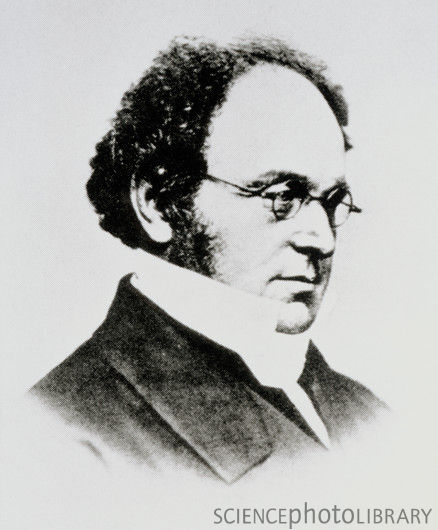
\includegraphics[width=0.5\textwidth]{figuren/verzamelingen_relaties/AugustusDeMorgan}
\caption{Augustus De Morgan (1806--1871)}
\label{fig:morgan}
\end{figure}

Er zijn twee wetten van de Morgan. De eerste wet stelt dat het complement van de unie van twee verzamelingen de doorsnede van de complementen is 
\begin{equation*}
\mathrm{Als~}X\subset U \mathrm{~en~} Y\subset U \mathrm{~dan~is~}  (X\union Y)^c=X^c \intersection  Y^c 
\end{equation*}
Als een element behoort tot de unie van twee verzamelingen $X$ en $Y$, hoort het tot $X$ \emph{of} tot $Y$. Als het element behoort tot het complement van de unie, behoort het \emph{niet} tot `$X$ of $Y$', dus hoort het niet tot $X$ \emph{en} niet tot $Y$. 

De tweede wet maakt een analoge redenering voor de doorsnede:  het complement van de doorsnede van twee verzamelingen is de unie van de complementen 
\begin{equation*}
 (X\intersection Y)^c=X^c \union  Y^c
\end{equation*}

\section{Productverzameling, paar en geordende $n$-tallen}\index{productverzameling}\index{verzameling!product-}\index{\ensuremath{\times}}
\label{sec:prodverz}
In het voorgaande vermeldden we reeds dat de elementen van een verzameling niet noodzakelijk enkelvoudig hoeven te zijn (bijvoorbeeld een getal of een letter), maar dat een verzameling ook kan bestaan uit andere verzamelingen. Dit kunnen we gebruiken om verzamelingen met  `gecombineerde' elementen te construeren. Voor een taak die studenten per twee moeten maken bijvoorbeeld kan je een verzameling maken van alle duo's. 

We weten dat de volgorde waarin elementen van een verzameling opgesomd worden niet van belang is: het duo $\{\mathrm{Piet},\mathrm{Els} \}$ is hetzelfde als het duo $\{\mathrm{Els},\mathrm{Piet} \}$. Als je voor de `gecombineerde' elementen van de verzameling dus opnieuw verzamelingen gebruikt, kan dat leiden tot verkeerde resultaten. Bijvoorbeeld, als je een verzameling wil maken waarbij elk element de combinatie is van postcode en bijhorend inwonersaantal, is het belangrijk dat je consequent bent en in elk element bijvoorbeeld het eerste getal de postcode voorstelt en het tweede getal het aantal inwoners. Je kan dus geen verzameling gebruiken om deze combinatie voor te stellen.  \label{pg:postcodes}

In de verzamelingenleer bestaat er een concept dat duo's van elementen uit verschillende verzamelingen samenstelt \'en de volgorde van die combinatie bewaart: de  productverzameling $X \times Y$. 

\begin{quote}

Het \emph{product} van twee verzamelingen $X$ en $Y$ is de verzameling van alle \emph{paren} $(x,y)$ waarbij $x\in X$ en $y\in Y$.
\begin{equation*}
X\times Y=\{(x,y)\mid x\in X ~\mathrm{en}~y\in Y\}
\end{equation*}

\end{quote}

In een paar $(x,y)$ is de volgorde belangrijk: $(x,y)\not =(y,x)$. Het paar $(x,y)=(a,b)$ als en slechts als $x=a$ en $y=b$.

Bijvoorbeeld: 
\begin{itemize}
\item als $X=\{1,2,3\}$ en $Y=\{a,b\}$, dan is 
\begin{equation*}
X\times Y=\{(1,a),(1,b),(2,a),(2,b),(3,a),(3,b) \}
\end{equation*}
\item Als $X=\real$ en $Y=\real$, dan is 
$X \times Y=\real^2$, de verzameling van alle koppels 
re\"ele getallen $(x,y)$. Deze verzameling ken je als het twee-dimensionale vlak.
\end{itemize}


Een productverzameling is niet beperkt tot het product van twee verzamelingen: je kan zoveel verzamelingen met mekaar vermenigvuldigen als nodig is:
\begin{quote}
De  productverzameling $A_1\times A_2\times\dots\times A_n$ van de verzamelingen $A_1$, $A_2$, \dots, $A_n$ is de verzameling van \emph{geordende $n$-tallen} (\emph{tupels}\index{tupel}) $(a_1,a_2,\dots,a_n)$ waarbij $a_1\in A_1$, $a_2\in  A_2$, \dots, $a_n \in A_n$.
\end{quote}
\begin{equation*}
A_1\times A_2\times\dots\times A_n=\{(a_1,a_2,\dots,a_n)\mid a_1\in A_1, a_2\in  A_2, \dots, a_n \in A_n\}
\end{equation*}

Als alle verzamelingen $A_1$, \dots, $A_n$ gelijk zijn, schrijven we het product van de verzamelingen als $A^n$.

Stel dat $A=\{\mathrm{a}, \mathrm{b},\dots,\mathrm{z}\}$, dan is $A^5$ de verzameling van alle `woorden' (strings) die bestaan uit kleine letters a-z met lengte 5. 
 
 
 
\newpage 
\section{Oefeningen}
\begin{oef}
Zijn de volgende verzamelingen goed gedefinieerd? Motiveer je antwoord.
\begin{enumerate}
\item De verzameling van de letters van het alfabet
\item De verzameling van grote mensen
\item De verzameling van re\"ele getallen waarvoor geldt $2x-9=16$
\item De verzameling van gehele getallen waarvoor geldt $2x-9=16$
\item De verzameling van goede voetballers
\end{enumerate}
\begin{opl}
\begin{enumerate}
\item Niet goed gedefinieerd: welk alfabet wordt er bedoeld? Zijn de hoofdletters ook element van de verzameling? Moet zijn: $\{\text{a},\text{b},\dots,\text{z},\text{A},\text{B},\dots,\text{Z}\}$
\item Niet goed gedefinieerd: wat is \emph{groot}? Moet zijn: verzameling van mensen groter dan \SI{1.80}{\meter}
\item Goed gedefinieerd
\item Goed gedefinieerd
\item Niet goed gedefinieerd: wat is \emph{goed}?
\end{enumerate}
\end{opl}
\end{oef}



\begin{oef}
Gegeven de verzameling $A=\{2,4,6,8,10\}$ en $B=\{1,3,6,7,8\}$. Welke uitspraken zijn waar? 
\begin{enumerate}
\item $2\in A$
\item $11\in B$
\item $4 \not \in B$
\item $\{2\}\in A$
\item $A\in \nat$
\item $A=\{x\mid x\in \nat \mathrm{~en~}x\mathrm{~is~even}\}$
\end{enumerate}
\begin{opl}
\begin{enumerate}
\item waar
\item niet waar
\item waar
\item niet waar: $\{2\}\subset A$ of $2\in A$
\item niet waar: $A\subset \nat$
\item niet waar: bijvoorbeeld $12\not \in A$. Zou wel waar zijn: $A=\{x\mid x\in \nat \mathrm{~en~}x\text{~is~even en }x\leqslant 10\}$
\end{enumerate}
\end{opl}
\end{oef}




\begin{oef}
Gegeven $A=\{4,\sqrt{2}, \frac{2}{3}, -2.5, -5,33,\sqrt{9},\pi \}$. Noteer volgende deelverzamelingen van $A$ door middel van opsomming:
\begin{enumerate}
\item De  getallen van $A$ die behoren tot $\nat$
\item De  getallen van $A$ die behoren tot $\integers$
\item De rationale getallen van $A$
\item De re\"ele getallen van $A$ die niet rationaal zijn
\end{enumerate}
\begin{opl}
\begin{enumerate}
\item $\{ 4,33,\sqrt{9}\}$
\item $\{ 4,33,\sqrt{9},-5\}$
\item $\{ 4,33,\sqrt{9},-5,\frac 23,-2.5\}$
\item $\{\sqrt{2},\pi\}$
\end{enumerate}
\end{opl}
\end{oef}



\begin{oef}
Waar of fout?
\begin{enumerate}
\item $\emptyset=\{0\}$
\item $x\subset \{x\}$
\item $\emptyset=\{\emptyset\}$
\item $\emptyset\in \{\emptyset\}$
\end{enumerate}
\begin{opl}
\begin{enumerate}
\item niet waar: $\emptyset=\{ \}$ of  $0\in \{0\}$ of $\emptyset\subset\{0\}$
\item niet waar: $x\in \{x\}$ of $\{x\}\subset \{x\}$
\item niet waar: $\emptyset\in\{\emptyset\}$ of $\emptyset\subset\{\emptyset\}$
\item waar
\end{enumerate}
\end{opl}
\end{oef}



\newpage
\begin{oef}
\label{oef:venndiagramoef}
Bekijk figuur~\ref{fig:venndiagramoef}. De getallen 1,\dots,8 duiden een deelverzameling aan van $U$. Vul  tabel~\ref{tab:venndiagram} aan. Als voorbeeld vulden we reeds de eerste lijn in.
\begin{figure}[htbp]
\centering
% oefening venn
\begin{tikzpicture}[thick]
\draw (-4,-2.7) rectangle (4,3.5) node [above] {$U$};
\draw \firstellipse node at (35:3.7cm) {$A$};
\draw \secondellipse node at (145:3.7cm) {$B$};
\draw \thirdellipse node at (270:2.3cm) {$C$};
\node at (0,3) {1};
\node at (1.8,1.3) {2};
\node at (0,1.5) {3};
\node at (-1.8,1.3) {4};
\node at (1,0) {5};
\node at (0,0.4) {6};
\node at (-1,0) {7};
\node at (0,-1) {8};
\end{tikzpicture}
\caption{8 gebieden in een Venndiagram}
\label{fig:venndiagramoef}
\end{figure}
\begin{table}[h!tbp]
\centering
\caption{Tabel bij figuur~\ref{fig:venndiagramoef}}
\begin{tabular}{ccccc}
\toprule
$\subset A$? & $\subset B$? & $\subset C$? & Gebied & in symbolen \\ 
\midrule
N & N & N & 1  & $(A \union B \union C)^c$ \\ 
N & N & J &  &   \\ 
N & J & N &   &   \\ 
N & J & J &   &   \\ 
J & N & N &   &   \\ 
J & N & J &   &   \\ 
J & J & N &   &   \\ 
J & J & J &   &   \\ 
\bottomrule
\end{tabular} 
\label{tab:venndiagram}
\end{table}

\begin{opl}
$\qquad$ \\
\begin{table}[h!tbp]
\centering
\caption{Oplossing van oefening~\ref{oef:venndiagramoef}}
\begin{tabular}{ccccc}
\toprule
$\subset A$? & $\subset B$? & $\subset C$? & Gebied & in symbolen \\ 
\midrule
N & N & N & 1  & $(A\union B \union C)^c$ \\ 
N & N & J & 8 & $C-(A\union B)$  \\ 
N & J & N &  4 & $B-(A\union C)$  \\ 
N & J & J &7   &$(B\intersection C)-A$   \\ 
J & N & N &  2 & $A-(B\union C)$  \\ 
J & N & J & 5  & $(A\intersection C)-B$  \\ 
J & J & N & 3  & $(A\intersection B)-C$  \\ 
J & J & J & 6  & $A\intersection B\intersection C$  \\ 
\bottomrule
\end{tabular} 
\label{tab:venndiagram2}
\end{table}

\end{opl}
\end{oef}




\begin{oef}
\label{oef:oefvenn}
Gegeven $U = \{1,2,3,4,5,6,7,8\}$, $P = \{3,6\}$,  $Q =\{1,3,4,5,6,8\}$ en $R = \{3,4,8\}$.
Teken  venndiagrammen voor deze verzamelingen en plaats de elementen waar ze horen. 
\begin{opl}
Het Venndiagram van figuur \ref{fig:UPQ} op pagina \pageref{fig:UPQ} toont de oplossing.
\begin{figure}[htbp]
\centering
    \begin{tikzpicture}[scale=0.8,thick]
    \draw (-4,-2.7) rectangle (4,3.5) node [above] {$U$};
	\draw (0,0.4) ellipse [x radius=3.6cm,y radius=2.6cm];
	\draw (-1.2,0.2) ellipse [x radius=1.8cm,y radius=1.3cm];
	\draw (1.2,0.2) ellipse [x radius=1.8cm,y radius=1.3cm];
	\node at (2.7,2.5) {$Q$};
	\node at (-2.3,1.5) {$P$};
	\node at (2.3,1.5) {$R$};
	\draw[fill] (0,2) \bol node [above] {1};
	\draw[fill] (3,-2.4) \bol node [above] {2};
	\draw[fill] (0,0) \bol node [above] {3};
	\draw[fill] (1,0.6) \bol node [above] {4};
	\draw[fill] (0,-1.8) \bol node [above] {5};
	\draw[fill] (-1.4,0) \bol node [above] {6};
	\draw[fill] (-3,-2) \bol node [above] {7};
	\draw[fill] (2,-0.3) \bol node [above] {8};
    \end{tikzpicture}
\caption{Oplossing bij oefening~\ref{oef:oefvenn}}
\label{fig:UPQ}
\end{figure}
\end{opl}
\end{oef}

\begin{oef}
Herneem de verzamelingen van oefening~\ref{oef:oefvenn}. Pas de bewerkingen $\intersection$, $\union$, $-$ en complement zo efficiënt mogelijk toe op de verzamelingen $P$, $Q$ en $R$ om volgende verzamelingen te omschrijven. De eerste oefening lossen we bij wijze van voorbeeld zelf op.
\begin{enumerate}
\item $\{2,7\}=Q^c$
\item $\{3\}$
\item $\{1,5\}$
\item $\{1,5,3\}$
\item $\{1,5,2,7\}$
\item $\{6,4,8\}$
\end{enumerate}
\begin{opl}
\item $\{2,7\}=Q^c$
\item $\{3\}=P\intersection R$
\item $\{1,5\}=Q-(P\union R)$ of $Q \intersection (P \union R)^c$
\item $\{1,5,3\}=(P\intersection R)\union (Q-(P\union R))$
\item $\{1,5,2,7\}=(P\union R)^c$
\item $\{6,4,8\}=(P\union R)- (P \intersection R)$
\end{opl}
\end{oef}


\begin{oef}
\label{oef:venndiagram3}
Teken venndiagrammen van de verzameling $U$, de deelverzamelingen $A$ en $B$ van $U$ en het element $x$ voor volgende gevallen:
\begin{enumerate}
\item $x\in A$ en $A\subset B$
\item $x\in A$ en $A$ en $B$ zijn disjunct
\item $x\in A$, $x\not \in B$, $B\subset A$
\end{enumerate}
\begin{opl}
De drie Venndiagrammen van figuur~\ref{fig:Venn3} op pagina~\pageref{fig:Venn3} tonen de oplossingen.
\begin{figure}[h!tbp]
\centering
\subfloat[oef a]{    \begin{tikzpicture}[scale=0.6,thick]
    \draw (-4,-2.7) rectangle (4,3.5) node [above] {$U$};
	\draw (0,0.4) ellipse [x radius=3.6cm,y radius=2.6cm];
	\node at (3,2.5) {$B$};
	\draw (-1.2,0.2) ellipse [x radius=1.8cm,y radius=1.3cm];
	\node at (0.2,1.5) {$A$};
	\draw[fill] (-1,0) \bol node [above] {$x$};
    \end{tikzpicture}}\qquad
\subfloat[oef b]{    \begin{tikzpicture}[scale=0.6,thick]
    \draw (-4,-2.7) rectangle (4,3.5) node [above] {$U$};
	\draw (1.6,0.3) ellipse [x radius=1.5cm,y radius=2.6cm];
	\node at (3,2.5) {$B$};
	\draw (-2,0.2) ellipse [x radius=1.4cm,y radius=2.4cm];
	\node at (-0.6,2) {$A$};
	\draw[fill] (-2,0) \bol node [above] {$x$};
    \end{tikzpicture}}\qquad
\subfloat[oef c]{    \begin{tikzpicture}[scale=0.6,thick]
    \draw (-4,-2.7) rectangle (4,3.5) node [above] {$U$};
	\draw (0,0.4) ellipse [x radius=3.6cm,y radius=2.6cm];
	\node at (3,2.5) {$A$};
	\draw (-1.2,0.2) ellipse [x radius=1.8cm,y radius=1.3cm];
	\node at (0.2,1.5) {$B$};
	\draw[fill] (2,0) \bol node [above] {$x$};
    \end{tikzpicture}}
\caption{Oplossingen bij oefening~\ref{oef:venndiagram3} }
\label{fig:Venn3}
\end{figure}
\end{opl}
\end{oef}



\begin{oef}
Gegeven de verzamelingen $A,B\subset U$. Duid aan op een venndiagram
\begin{enumerate}
  \item $(A^c)^c \union B$
  \item $A\intersection  B^c$
  \item $(A\intersection B)^c$
  \item $A^c \union  B^c$
  \item $(A\union B)^c$
  \item $A^c \intersection B^c$
\end{enumerate}

\begin{opl}
{
\def\labels{
  \node[anchor=south east] at (-1.55,.6) {$A$};
  \node[anchor=south west] at (1.55,.6) {$B$};
}
\def\universe{(-2.5,-1.5) rectangle +(5,3)}
\def\ellA{(-.9,0) ellipse (1.25cm and 0.75cm)}
\def\ellB{(.9,0) ellipse (1.25cm and 0.75cm)}
\pgfkeys{/tikz/.cd,
         highlight/.style={fill=gray!30},
         empty/.style={fill=white},
         outline/.style={fill=none}}

\begin{center}
\begin{tabular}{cc}
  1.
  \begin{tikzpicture}
    \draw[thick] \universe;
    \draw[highlight] \ellA;
    \draw[highlight] \ellB;
    \draw[outline] \ellA;
    \labels
  \end{tikzpicture}
  &
  2.
  \begin{tikzpicture}
    \draw[thick] \universe;
    \draw[highlight] \ellA;
    \draw[empty] \ellB;
    \draw[outline] \ellA;
    \labels
  \end{tikzpicture}
  \\
  3.
  \begin{tikzpicture}
    \draw[thick,highlight] \universe;
    \begin{scope}
      \clip \ellA;
      \clip \ellB;
      \draw[empty] \ellA;
    \end{scope}

    \draw[outline] \ellA;
    \draw[outline] \ellB;
    \labels
  \end{tikzpicture}
  &
  4.
  \begin{tikzpicture}
    \draw[thick,highlight] \universe;
    \begin{scope}
      \clip \ellA;
      \clip \ellB;
      \draw[empty] \ellA;
    \end{scope}

    \draw[outline] \ellA;
    \draw[outline] \ellB;
    \labels
  \end{tikzpicture}
  \\
  5.
  \begin{tikzpicture}
    \draw[thick,highlight] \universe;
    \draw[empty] \ellA;
    \draw[empty] \ellB;
    \draw[outline] \ellA;
    \labels
  \end{tikzpicture}
  &
  6.
  \begin{tikzpicture}
    \draw[thick,highlight] \universe;
    \draw[empty] \ellA;
    \draw[empty] \ellB;
    \draw[outline] \ellA;
    \labels
  \end{tikzpicture}
\end{tabular}
\end{center}
}
\end{opl}
\end{oef}



\begin{oef}
Zij $A$,$B$,$C$ en $D$ verzamelingen. Bepaal of de volgende beweringen waar of onwaar zijn. Toon je antwoord aan met venndiagrammen.
\begin{enumerate}
  \item Als $C\subset D^c$, dan is $D \not \subset C^c$
  \item Als $C\not \subset D$, dan is $D^c \not \subset C^c$
  \item Als $A\subset B$, dan is $A\intersection B =A$
\end{enumerate}
\begin{opl}
\begin{enumerate}
  \item niet waar: als $D \not \subset C^c$, is er  een element van $D$ dat geen element is van $C^c$, dus element is van $C$. Dan hebben we een element van $C$ gevonden dat tevens element is van $D$.
  \item waar
  \item waar
\end{enumerate}
\end{opl}
\end{oef}


\begin{oef}
Geef door opsomming
\begin{enumerate}
  \item $A=\{x \in \real | (x-1)\cdot(x-2)=6\}$
  \item $B=\{10\cdot x|x\in\integers \}$
  \item $C=\{ x\in \nat| x \textrm{ is een deler van } 6\}$
  \item $U = \{(x, y) \in A \times B|y = 2\cdot x + 10\}$ waarbij $A = \{0,1,2,\cdots,6\}$ en \\$B = \{10,11,12,\dots,20\}$
  \item $V = \{(x, y) \in A \times B|y = x - 10\}$ waarbij  $A = \{10,11,12,\dots,20\}$ en \\ $B = \{0,1,2,\cdots,6\}$
  \item $W = \{(x, y) \in A \times  B|y = \sqrt{x}\}$ waarbij $A=\{-4,-1,0,1,4,9\}$ en \\ 
        $B=\{-3,-2,-1,0,1,2,3\}$
\end{enumerate}
\begin{opl}
\begin{enumerate}
  \item $A=\{4,-1\}$
  \item $B=\{0,10,-10,20,-20,\dots\}$
  \item $C=\{1,2,3,6\}$
  \item $U=\{(0,10),(1,12),(2,14),(3,16),(4,18),(5,20)\}$
  \item $V=\{(10,0),(11,1),\dots, (16,6\}$
  \item $W=\{(0,0),(1,1),(4,2),(9,3)\}$
\end{enumerate}
\end{opl}
\end{oef}




\newpage
\begin{oef}
Hieronder vind je de verzameling $U$ en de deelverzamelingen $P$, $Q$ en $R$ van $U$. Pas de bewerkingen $-$, $\intersection$, $\union$ en complement zo effici\"ent mogelijk toe op de \emph{deel}verzamelingen van $U$ om \emph{het grijze gedeelte} te omschrijven.
\begin{multicols}{2}
\begin{enumerate}

\begin{minipage}{\columnwidth}
\item
\centering
%\vspace{-0.4cm}
\begin{tikzpicture}[scale=0.7,thick]
  \path[use as bounding box] (-4,-3) rectangle (4,4);
  \filldraw[fill=gray!30] (-4,-3) rectangle (4,3.5) node [above] {$U$};
  \fill[white] \firstellipse;
  \fill[white] \secondellipse;
  \fill[fill=gray!30] \thirdellipse;
  \draw \firstellipse node at (35:3.7cm) {$Q$};
  \draw \secondellipse node at (145:3.7cm) {$P$};
  \draw \thirdellipse node at (270:2.3cm) {$R$};
\end{tikzpicture}
\end{minipage}

\begin{minipage}{\columnwidth}
\item
\centering
%\vspace{-0.4cm}
\begin{tikzpicture}[scale=0.7,thick]
  \draw (-4,-3) rectangle (4,3.5) node [above] {$U$};
  \begin{scope}
    \clip \secondellipse;
    \fill[gray!30] \thirdellipse;
  \end{scope}
  \begin{scope}
    \clip \firstellipse;
    \fill[gray!30] \thirdellipse;
  \end{scope}
  \draw \firstellipse node at (35:3.7cm) {$Q$};
  \draw \secondellipse node at (145:3.7cm) {$P$};
  \draw \thirdellipse node at (270:2.3cm) {$R$};
\end{tikzpicture}
\end{minipage}

\begin{minipage}{\columnwidth}
\item
\centering
%\vspace{-0.4cm}
\begin{tikzpicture}[scale=0.7,thick]
  \filldraw[fill=gray!30] (-4,-3) rectangle (4,3.5) node [above] {$U$};
  \begin{scope}
    \clip \secondellipse;
    \fill[white] \firstellipse;
  \end{scope}
  \fill[gray!30] \thirdellipse;
  \draw \firstellipse node at (35:3.7cm) {$Q$};
  \draw \secondellipse node at (145:3.7cm) {$P$};
  \draw \thirdellipse node at (270:2.3cm) {$R$};
\end{tikzpicture}
\end{minipage}

\begin{minipage}{\columnwidth}
\item
\centering
%\vspace{-0.4cm}
\begin{tikzpicture}[scale=0.7,thick]
  \draw (-4,-3) rectangle (4,3.5) node [above] {$U$};
  \begin{scope}
    \clip \secondellipse;
    \fill[gray!30] \thirdellipse;
  \end{scope}
  \fill[gray!30] \firstellipse;
  \draw \firstellipse node at (35:3.7cm) {$Q$};
  \draw \secondellipse node at (145:3.7cm) {$P$};
  \draw \thirdellipse node at (270:2.3cm) {$R$};
\end{tikzpicture}
\end{minipage}

\begin{minipage}{\columnwidth}
\item
\centering
%\vspace{-0.4cm}
    \begin{tikzpicture}[scale=0.7,thick]
    \draw (-4,-2.7) rectangle (4,3.5) node [above] {$U$};
    \fill[gray!30] \secondellipse;
    \fill[white] \firstellipse;
    \fill[white] \thirdellipse;     
    \draw \firstellipse node at (35:3.7cm) {$Q$};
    \draw \secondellipse node at (145:3.7cm) {$P$};
    \draw \thirdellipse node at (270:2.3cm) {$R$};
    \end{tikzpicture}
\end{minipage}

\begin{minipage}{\columnwidth}
\item
\centering
%\vspace{-0.4cm}
\begin{tikzpicture}[scale=0.7,thick]
  \filldraw[fill=gray!30] (-4,-3) rectangle (4,3.5) node [above] {$U$};
  \begin{scope}
    \clip \secondellipse;
    \clip \thirdellipse;
    \fill[white] \firstellipse;
  \end{scope}
  \draw \firstellipse node at (35:3.7cm) {$Q$};
  \draw \secondellipse node at (145:3.7cm) {$P$};
  \draw \thirdellipse node at (270:2.3cm) {$R$};
\end{tikzpicture}
\end{minipage}

\end{enumerate}
\end{multicols}

\begin{opl}
\begin{enumerate}
\item $\left(\left(P\union Q\right)-R\right)^c$
\item $\left(P\union Q\right) \intersection R$
\item $\left(\left(P\intersection Q\right)-R\right)^c$
\item $(P\intersection R)\union Q$
\item $P-(Q\union R)$
\item $(P\intersection Q \intersection R)^c$
\end{enumerate}
\end{opl}
\end{oef}



\newpage
\begin{oef}
\label{oef:oefLeentje}
%\begin{figure}[htb]
%\centering
%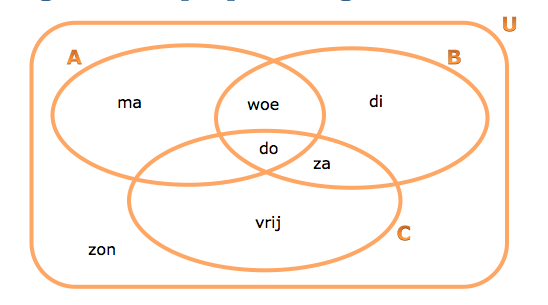
\includegraphics[width=0.7\textwidth]{figuren/verzamelingen_relaties/oefeningLeentje}
%
%\end{figure}
Zij $U$ de dagen van vorige week; $A$ de dagen met zon; $B$ de dagen met kou; $C$ de dagen met regen (figuur~\ref{fig:dagen}).
\begin{figure}[htbp]
\centering
% oefening venn
\begin{tikzpicture}[thick]
\draw (-4,-2.7) rectangle (4,3.5) node [above] {$U$};
\draw \firstellipse node at (35:3.7cm) {$B$};
\draw \secondellipse node at (145:3.7cm) {$A$};
\draw \thirdellipse node at (270:2.3cm) {$C$};
\node at (0,3) {zo};
\node at (1.8,1.3) {di};
\node at (0,1.5) {wo};
\node at (-1.8,1.3) {ma};
\node at (1,0) {za};
\node at (0,0.4) {do};
\node at (0,-1) {vr};
\end{tikzpicture}
\caption{Dagen van vorige week, figuur bij oefening~\ref{oef:oefLeentje}}
\label{fig:dagen}
\end{figure}
\begin{enumerate}
\item Geef door omschrijving:
\begin{enumerate}
\item $A\intersection B$
\item $(A\intersection C)-B$
\item $(A\union C)-B$
\item $A^c\intersection B^c$
\item $B^c\intersection C$
\end{enumerate}
\item Geef door opsomming:
\begin{enumerate}
\item $B-(A\intersection C)$
\item $C-(A\union B)$
\item $(A\union C)^c-B$
\item $(A-C)^c$
\end{enumerate}
\item Duid aan op het venndiagram:
\begin{enumerate}
\item $A^c-C$
\item $B^c -C$
\item $(A-C)^c$
\end{enumerate}
\end{enumerate}

\begin{opl}
\begin{enumerate}
\item \begin{enumerate}
\item $\{x| x \text{ is een dag met zon en kou} \}$
\item $\{x| x \text{ is een dag met zon en regen maar zonder kou} \}$
\item $\{x| x \text{ is een dag met zon of regen maar zonder kou} \}$
\item $\{x| x \text{ is een dag zonder zon en zonder kou} \}$
\item $\{x| x \text{ is een dag zonder kou en met regen} \}$
\end{enumerate}
\item \begin{enumerate}
\item $\{\text{di},\text{wo},\text{za} \}$
\item $\{\text{vr} \}$
\item $\{ \text{zo}\}$
\item $\{ \text{di},\text{do},\text{vr},\text{za},\text{zo}\}$
\end{enumerate}
\end{enumerate}
\end{opl}
\end{oef}

%%% Local Variables: 
%%% mode: latex
%%% TeX-master: "cursusTW1"
%%% End: 
